\documentclass[12pt]{article}

\usepackage[utf8]{inputenc}
\usepackage{latexsym,amsfonts,amssymb,amsthm,amsmath}
\usepackage{float}

\setlength{\parindent}{0in}
\setlength{\oddsidemargin}{0in}
\setlength{\textwidth}{6.5in}
\setlength{\textheight}{8.8in}
\setlength{\topmargin}{0in}
\setlength{\headheight}{18pt}
\usepackage{graphicx}

\usepackage{hyperref}
\hypersetup{
    colorlinks=true,
    linkcolor=blue,
    filecolor=magenta,      
    urlcolor=cyan,
    pdftitle={Overleaf Example},
    pdfpagemode=FullScreen,
    }

\urlstyle{same}

\usepackage{caption}
\DeclareCaptionFormat{citation}{%
  \ifx\captioncitation\relax\relax\else
    \captioncitation\par
  \fi
  #1#2#3\par}
\newcommand*\setcaptioncitation[1]{\def\captioncitation{\textit{Source:}~#1}}
\let\captioncitation\relax
\captionsetup{format=citation,justification=centering}


\title{MATH1034OL1 Pre-Calculus Mathematics Midterm Review (Wednesday)}
\author{Elijah Renner}

\begin{document}

\maketitle

\vspace{0.5in}

\tableofcontents

\section{About Today's Notes}

Since we didn't cover any new content Wednesday, I'm compiling all key information for the midterm here.

\section{Identities}

\subsection{Pythagorean Identities}

We first derive the identity \(\cos^2\theta + \sin^2\theta = 1\) from the unit circle.\\

\begin{figure}[H]
	\centering
	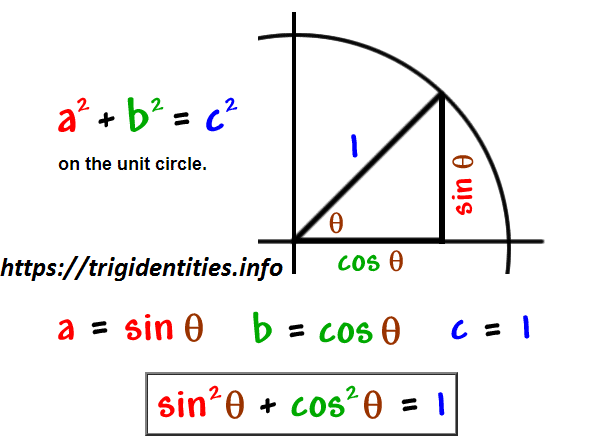
\includegraphics[scale=0.4]{Pythagorean Identity.png}
	\caption{Credit: \url{https://trigidentities.info/pythagorean-trig-identities}}
\end{figure}

Then, the other two Pythagorean identities are derived by dividing by either \(\cos^2\) or \(\sin^2\):\\

To derive \(\tan^2\theta+1=\sec^2\theta\), divide the original identity by \(\cos^2\theta\):\\

\[\frac{\cos^2\theta + \sin^2\theta = 1}{\cos^2\theta}\implies\frac{\cos^2\theta}{\cos^2\theta}+\frac{\sin^2\theta}{\cos^2\theta}=\frac{1}{\cos^2\theta}\implies\tan^2\theta+1=\sec^2\theta\]

To derive \(\cot^2\theta+1=\csc^2\theta\), divide the original identity by \(\sin^2\theta\):\\

\[\frac{\cos^2\theta + \sin^2\theta = 1}{\sin^2\theta}\implies\frac{\cos^2\theta}{\sin^2\theta}+\frac{\sin^2\theta}{\sin^2\theta}=\frac{1}{\sin^2\theta}\implies\cot^2\theta+1=\csc^2\theta\]

To summarize, the three Pythagorean identities are 

\begin{enumerate}
	\item \(\cos^2\theta + \sin^2\theta = 1\)
	\item \(\tan^2\theta+1=\sec^2\theta\)
	\item  \(\cot^2\theta+1=\csc^2\theta\)
\end{enumerate}

\subsection{Sum and Difference Formulas}

The sum and difference formulas allow us to evaluate the trigonometric functions of angles whos reference angles aren't 30, 45, 60, or 90:\\

\[\sin(A\pm B)=\sin A\cdot\cos B \pm \cos A\cdot\sin B\]

\[\cos(A\pm B)=\cos A\cdot\cos B \mp \sin A\cdot\sin B\]

There is a formula for \(\tan(A\pm B)\), which isn't necessary to remember, as it can be derived from \(\frac{\sin(A\pm B)}{\cos(A\pm B)}\) since \(\tan\theta=\frac{\sin\theta}{\cos\theta}\). The same follows for \(\csc(A\pm B)=\frac{1}{\sin(A\pm B)}\), \(\sec(A\pm B)=\frac{1}{\csc(A\pm B)}\), and \(\cot(A\pm B)=\frac{\cos(A\pm B)}{\sin(A\pm B)}\).\\

Regardless, \\

\[\tan(A\pm B)=\frac{\tan A\pm \tan B}{1\mp\tan A\cdot\tan B}\].

Also, \(\mp\) indicates the opposite sign of whichever sign is chosen as \(\pm\).

\subsection{Double Angle Formulas}

To derive the double angle formulas, we start with the angle familiar sum identities.

\subsubsection{Sine}

The angle sum identity for sine is:
\[
\sin(A + B) = \sin A \cos B + \cos A \sin B
\]

By setting \(A = B = \theta\), we get:
\[
\sin(2\theta) = \sin(\theta + \theta) = \sin \theta \cos \theta + \cos \theta \sin \theta
\]

Simplify this by combining like terms:
\[
\sin(2\theta) = 2 \sin \theta \cos \theta
\]

\subsubsection{Cosine}

The angle sum identity for cosine is:
\[
\cos(A + B) = \cos A \cos B - \sin A \sin B
\]

By setting \(A = B = \theta\), we get:
\[
\cos(2\theta) = \cos(\theta + \theta) = \cos \theta \cos \theta - \sin \theta \sin \theta
\]

Simplify this by combining like terms:
\[
\cos(2\theta) = \cos^2 \theta - \sin^2 \theta
\]

Using the Pythagorean identity \(\sin^2 \theta + \cos^2 \theta = 1\), we can derive alternative forms of \(\cos(2\theta)\):\\

1. Express \(\cos^2 \theta\) in terms of \(\sin^2 \theta\):
\[
\cos^2 \theta = 1 - \sin^2 \theta
\]

Substitute this into the double angle formula for cosine:
\[
\cos(2\theta) = (1 - \sin^2 \theta) - \sin^2 \theta = 1 - 2 \sin^2 \theta
\]

2. Express \(\sin^2 \theta\) in terms of \(\cos^2 \theta\):
\[
\sin^2 \theta = 1 - \cos^2 \theta
\]

Substitute this into the double angle formula for cosine:
\[
\cos(2\theta) = \cos^2 \theta - (1 - \cos^2 \theta) = 2 \cos^2 \theta - 1
\]

So, we have three equivalent forms of \(\cos(2\theta)\):
\[
\cos(2\theta) = \cos^2 \theta - \sin^2 \theta = 1 - 2 \sin^2 \theta = 2 \cos^2 \theta - 1
\]

These derivations give us the double angle formulas for sine and cosine:
\[
\sin(2\theta) = 2 \sin \theta \cos \theta
\]

\begin{align*}
\cos(2\theta) &= \cos^2 \theta - \sin^2 \theta \\
  &= 1 - 2 \sin^2 \theta \\
  &= 2 \cos^2 \theta - 1
\end{align*}


Nice!

\subsection{Half Angle Formulas}

The half angle formulas for \(\sin\) and \(\cos\) are\\
  
\[
\sin^2\theta = \frac{1}{2}(1 - \cos(2\theta)) \implies \sin\theta = \pm \sqrt{\frac{1}{2}\left(1 - \cos(2\theta)\right)} = \pm \sqrt{\frac{1 - \cos(2\theta)}{2}}
\]

\[
\cos^2\theta = \frac{1}{2}(1 + \cos(2\theta)) \implies \cos\theta = \pm \sqrt{\frac{1}{2}\left(1 + \cos(2\theta)\right)} = \pm \sqrt{\frac{1 + \cos(2\theta)}{2}}
\]\\

To derive the half-angle formula for \(\tan\), we use the half-angle formulas for \(\sin\) and \(\cos\):
\[
\tan \theta = \frac{\sin \theta}{\cos \theta}
\]

Using the half-angle formulas:
\[
\sin \theta = \pm \sqrt{\frac{1 - \cos(2\theta)}{2}}
\]
\[
\cos \theta = \pm \sqrt{\frac{1 + \cos(2\theta)}{2}}
\]

So,
\[
\tan \theta = \frac{\sin \theta}{\cos \theta} = \frac{\pm \sqrt{\frac{1 - \cos(2\theta)}{2}}}{\pm \sqrt{\frac{1 + \cos(2\theta)}{2}}}
\]

Since both the numerator and the denominator have the same sign, the signs cancel out:
\[
\tan \theta = \sqrt{\frac{1 - \cos(2\theta)}{2}} \div \sqrt{\frac{1 + \cos(2\theta)}{2}} = \sqrt{\frac{1 - \cos(2\theta)}{1 + \cos(2\theta)}}
\]

Thus, the half-angle formula for \(\tan\) is:
\[
\tan \theta = \sqrt{\frac{1 - \cos(2\theta)}{1 + \cos(2\theta)}}
\]

\section{Polynomial Behavior}

If a factor \((x-a)\) appears an even amount of times, the function will touch the x-axis when \(x=a\).\\

Conversely, if \((x-a)\) appears an odd amount of times, the function will cross the x-axis when \(x=a\):

\begin{figure}[H]
	\centering
	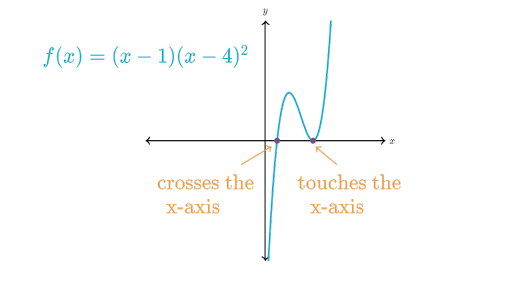
\includegraphics[scale=1]{Polynomial touching.png}
	\caption{Credit: \url{https://www.khanacademy.org/math/algebra2/x2ec2f6f830c9fb89:poly-graphs/x2ec2f6f830c9fb89:poly-intervals/a/zeros-of-polynomials-and-their-graphs}}
\end{figure}

\section{Quadrant of Manipulated Angle}

Problem: if angle \(\theta\) is in quadrant four, which quadrant is \(\frac{\theta}{2}\) in?\\

We know that a point on an axis is not in a quadrant, so the range of \(\theta\) is \(270^{\circ}<\theta<360^{\circ}\) or \(\frac{3\pi}{2}<\theta<2\pi\). To find the range of \(\frac{\theta}{2}\), treat \(\frac{3\pi}{2}<\theta<2\pi\) as an inequality. \\

Recall that we can divide each part of an inequality by a non-negative number without changing its sides. So, we'll divide by 2 to get \(\frac{\theta}{2}\) in the center:

\[\frac{3\pi}{4}<\frac{\theta}{2}<\pi\]

Since this range is in quadrant two, we know \(\frac{\theta}{2}\) must be in quadrant two.

\section{Absolute Value Equations}

\begin{figure}[H]
	\centering
	\includegraphics[width=\textwidth]{Absolute Value Equations Image.gif}
	\caption{Credit: \url{https://superbiamk.shop/product_details/85110602.html}}
\end{figure}

\section{Root Equations}

\begin{figure}[H]
	\centering
	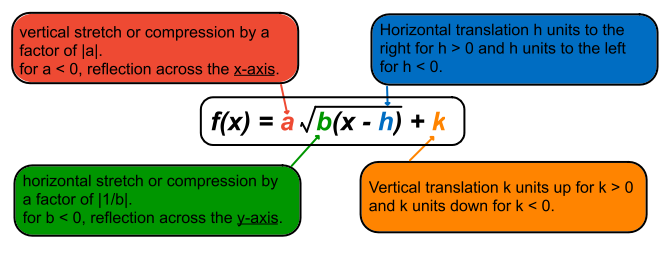
\includegraphics[width=\textwidth]{Root Functions Screenshot Aug 26.png}
	\caption{Credit: \url{https://amandapaffrath.weebly.com/square-root-functions.html}}
\end{figure}

\section{Sinusoidal Functions}

\begin{figure}[H]
	\centering
	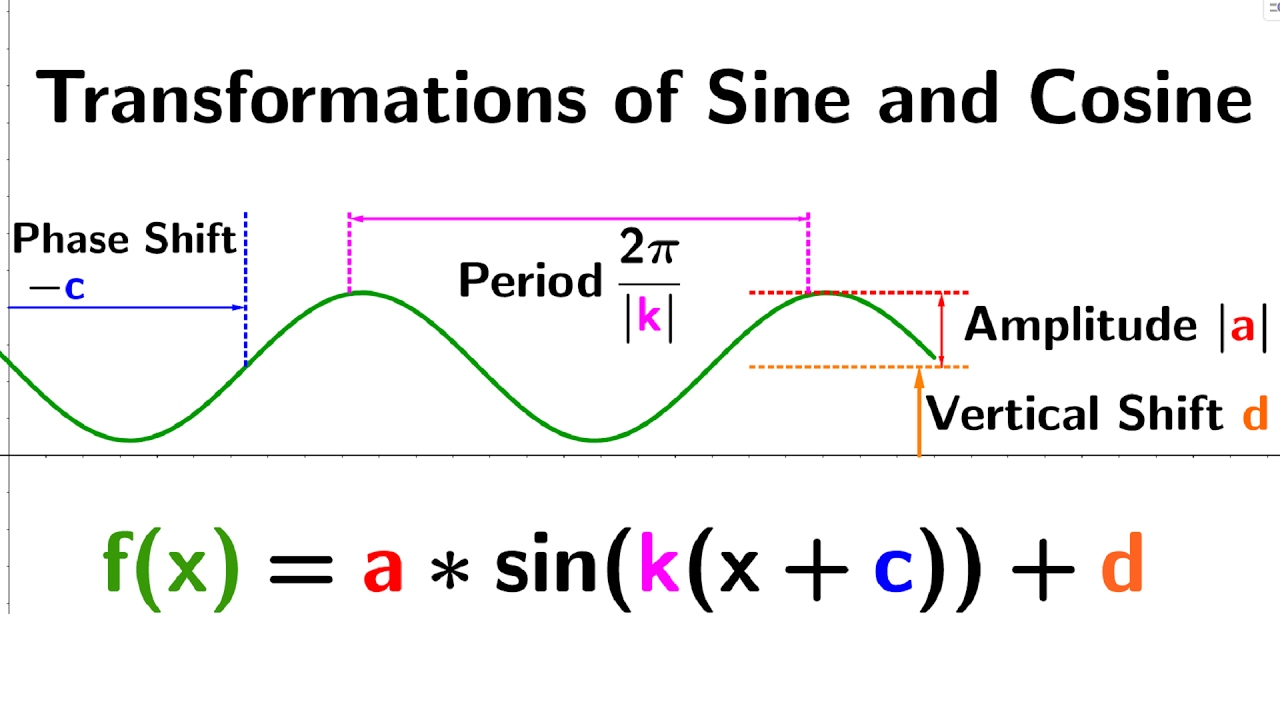
\includegraphics[width=\textwidth]{maxresdefault.jpg}
	\caption{Credit: \url{https://www.youtube.com/watch?v=AS7THLj-OhI}}
\end{figure}

\section{Domain}

\subsection{Domain of Root Functions}

\begin{figure}[H]
	\centering
	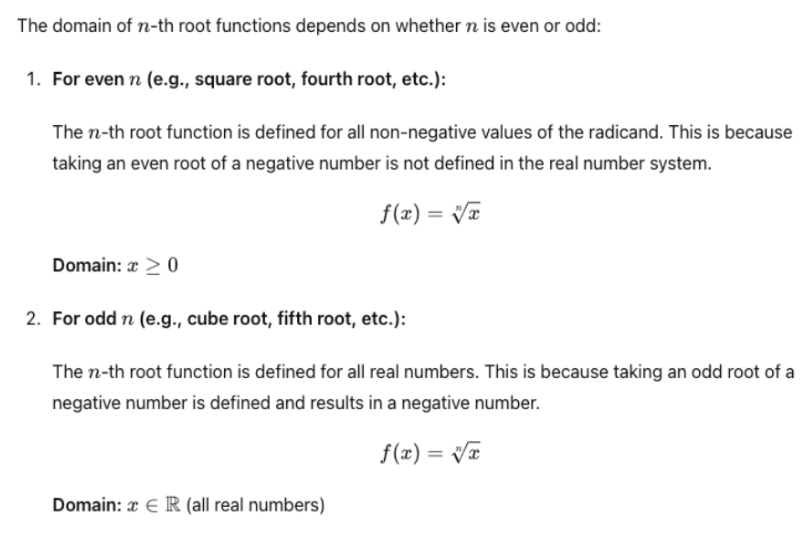
\includegraphics[width=\textwidth]{root.png}
	\caption{Credit: myself}
\end{figure}

\subsection{Domain of Polynomials}

All \(n\)-th degree polynomials in the  form \(a_nx^n+a_{n-1}x^{n-1}...+a_2x^2+a_1x+a_0\) are defined for all \(x\in\mathbb{R}\).

\subsection{Domain of Rational Functions}

Rational functions \(\frac{f(x)}{p(x)}\) are defined for all values where \(p(x)\neq0\).

\subsection{Domain of Added, Subtracted, Multiplied, and Divided Functions}

\begin{figure}[H]
	\centering
	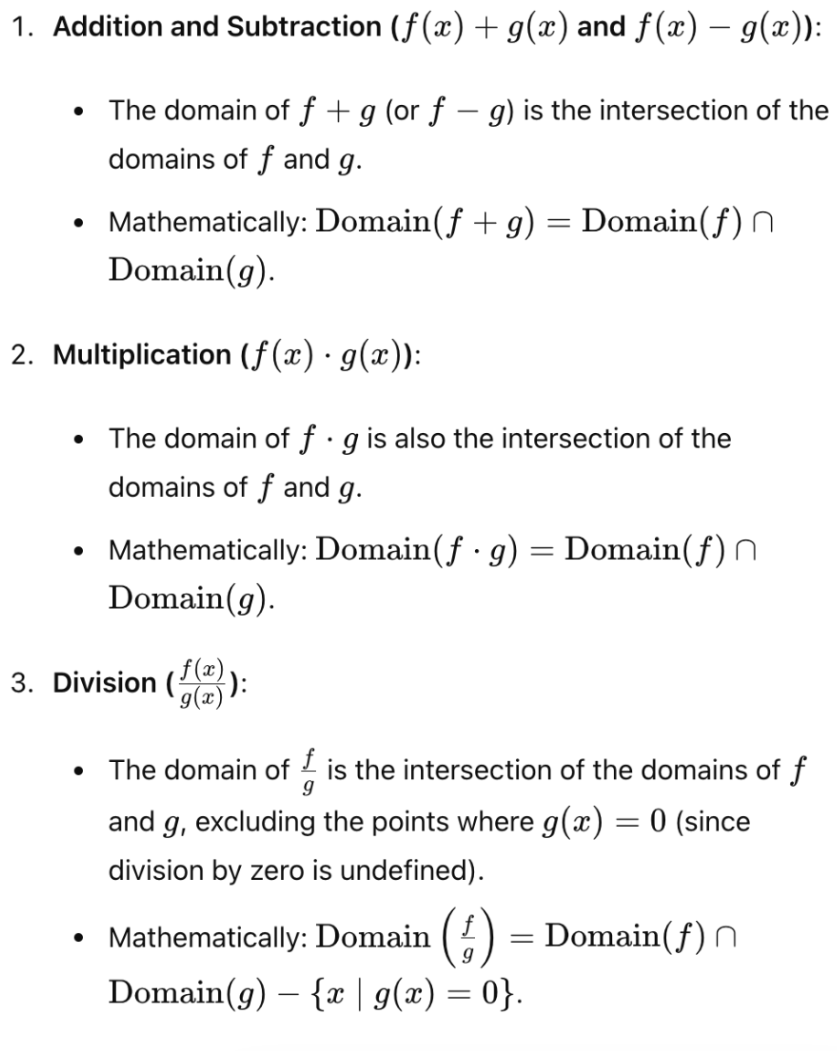
\includegraphics[scale=0.35]{add.png}
	\caption{Credit: myself}
\end{figure}

\subsection{Domain of Composed Functions}

Here's a review of set builder notation:

\begin{figure}[H]
	\centering
	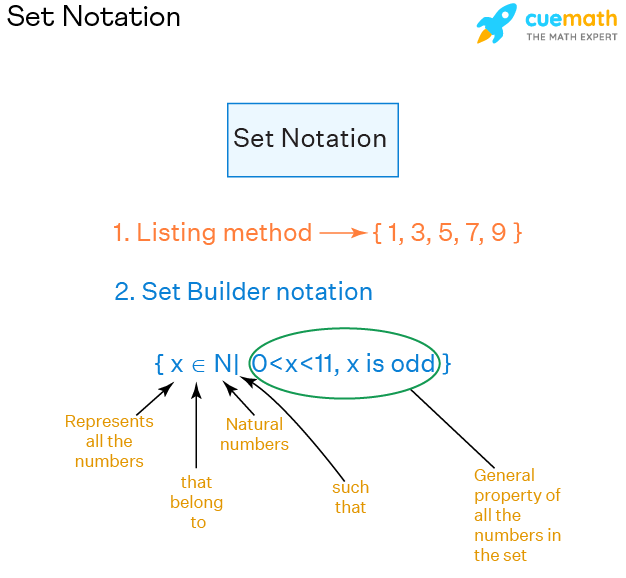
\includegraphics[scale=0.35]{sets.png}
	\caption{Credit: \url{https://www.cuemath.com/algebra/set-builder-notation/}}
\end{figure}

\[\text{Domain}(g\circ f)=\left\{x\in\text{Domain}(g)\text{ }|\text{ }g(x)\in\text{Domain}(f)\right\}\]

\section{Limit Definition of the Derivative}

The derivative (or instantaneous rate of change) of a function \(f\) at a point \( x = a \) is defined by the limit:

\[
f'(a) = \lim_{{h \to 0}} \frac{f(a+h) - f(a)}{h}
\]

\section{Rationalizing Numerator and Denominator}

\begin{figure}[H]
	\centering
	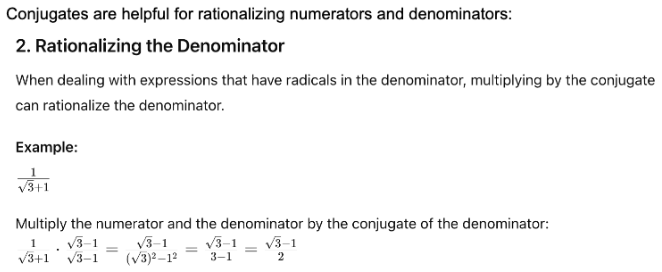
\includegraphics[width=\textwidth]{denominator}
	\caption{Credit: myself}
\end{figure}

\section{Inverse Functions}

\subsection{Finding Inverses}
Given a function \(f(x)\), we denote its inverse as \(f^{-1}(x).\) To find the inverse of \(f(x)\):\\

\begin{enumerate}
  \item Replace \(f(x)\) with \(y\).
  \item Switch \(y\) and \(x\).
  \item Solve for \(y\).
  \item Replace \(y\) with \(f^{-1}(x)\)
\end{enumerate}

Here's an example:\\

Problem: Let \(f(x)=x^2+3\). Find \(f^{-1}(x)\).\\

Replace \(f(x)\) with \(y\): \(f(x)=x^2+3\implies y=x^2+3\)\\

Switch \(x\) and \(y\): \(y=x^2+3\implies x=y^2+3\)\\

Solve for \(y\): \(x=y^2+3\implies y^2=x-3 \implies y=\sqrt{x-3}\)\\

Replace \(y\) with \(f^{-1}(x)\): \(f^{-1}(x)=\sqrt{x-3}\)\\

Now we know \(f^{-1}(x)=\sqrt{x-3}\).\\

\subsection{Properties of Inverses}

A cool property of inverse functions is that \(f(x)\) and \(f^{-1}(x)\) reflect over the line \(y=x\):\\

\begin{figure}[H]
	\centering
	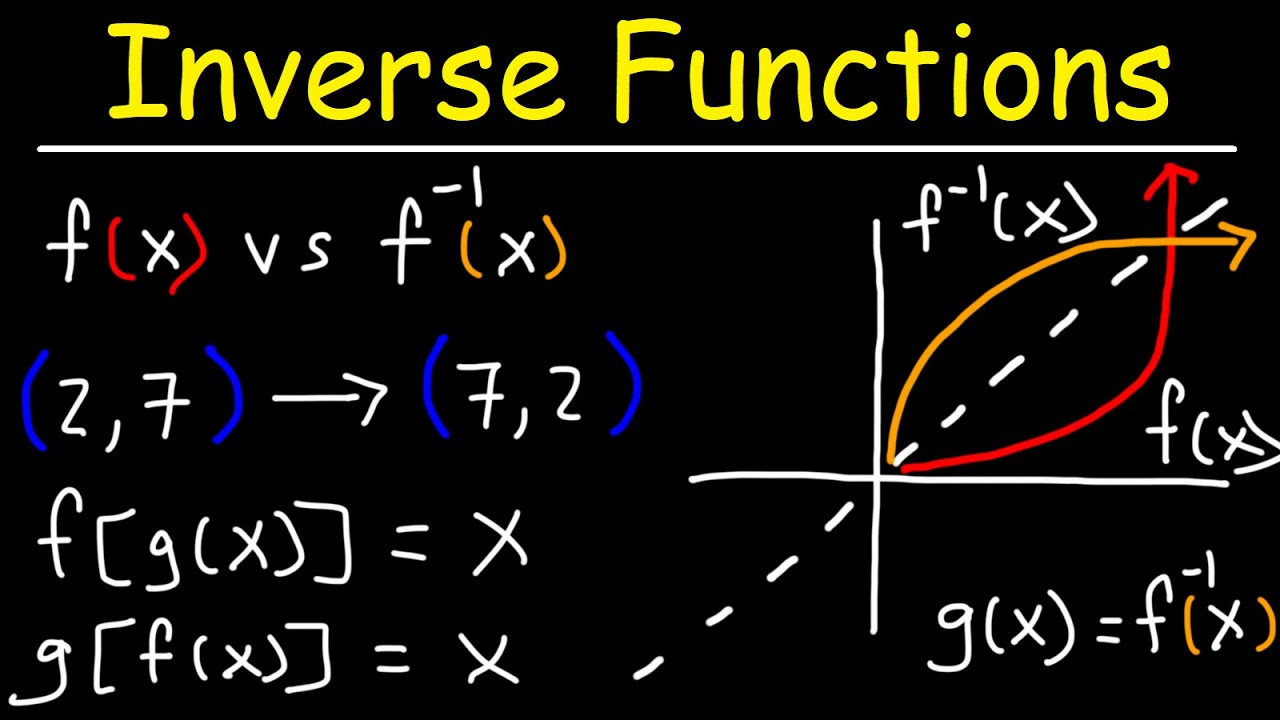
\includegraphics[scale=0.2]{inverse.jpg}
	\caption{Credit: \url{https://youtu.be/TN4ybFiuV3k}}
\end{figure}

This makes sense because we are switching \(x\) and \(y\).\\

Another property of \(f^{-1}\) is that its domain and range are the range and domain respectfully of \(f\). More formally:\\

\(\text{domain}(f)=\text{range}(f^{-1})\)\\

\(\text{range}(f)=\text{domain}(f^{-1})\)\\

\section{Review of Linear Functions}

To find the slope of a line given two points, we use \(slope = m = \frac{\Delta y}{\Delta x}\). Given two points \((x_1,y_1) \text{ and } (x_2, y_2)\), we can calculate the slope using\\

\[\frac{y_1-y_2}{x_1-x_2}\]

If we a line's slope \(m\) and a point \((x_1,y_1)\) on the line, we can write its equation as\\

\[y-y_1=m(x-x_1)\]

Some rules:\\
A line parallel to a line with slope \(m\) will have slope \(m\)\\
A line perpendicular to a line with slope \(m\) will have slope \(-\frac{1}{m}\)\\
A line written in the form \(Ax+By=C\) will have slope \(m=-\frac{A}{B}\) and y-intercept \(b=\frac{C}{B}\)\\

\section{End Behaviors}

\begin{figure}[H]
	\centering
	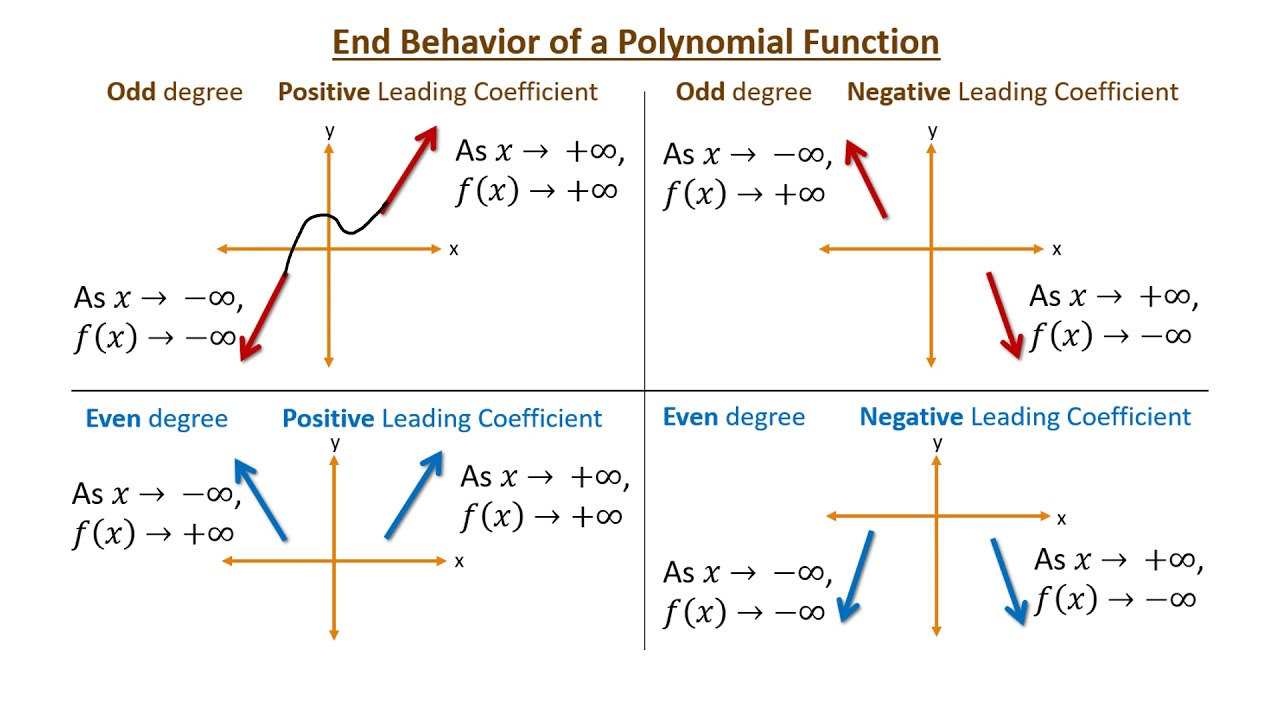
\includegraphics[scale=0.4]{ends.jpg}
	\caption{Credit: \url{https://youtu.be/7LnsYtCfkXQ?si=Iq8WqdaHbLvWcLC0}}
\end{figure}

\section{Transformations of Functions}

Here's a helpful graphic about transforming functions:

\begin{figure}[H]
	\centering
	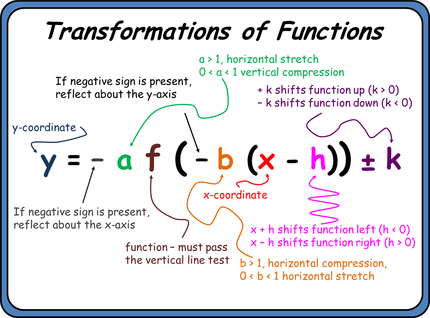
\includegraphics[scale=0.5]{9546920.png}
	\caption{Credit: \url{https://lzinnick.weebly.com/transformations-of-functions-and-graphs.html}}
\end{figure}

\section{Special Triangles}

\begin{figure}[H]
	\centering
	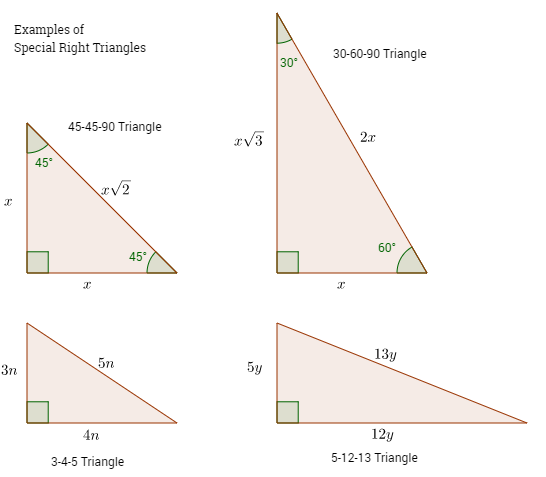
\includegraphics[scale=0.5]{triangles.png}
	\caption{Credit: \url{https://www.onlinemathlearning.com/special-right-triangles.html}}
\end{figure}


\section{All Students Take Calculus}

"All Students Take Calculus." tells us which trig functions are positive in each quadrant.\\

\begin{figure}[ht]
	\centering
	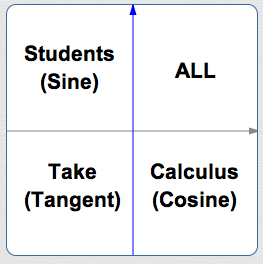
\includegraphics[scale=.75]{memoryDeviceSigns}
	\caption{Credit: \url{https://www.onemathematicalcat.org}}
\end{figure}

\section{Finding the Radius and Center of Circle by Completing the Square}



\begin{figure}[ht]
	\centering
	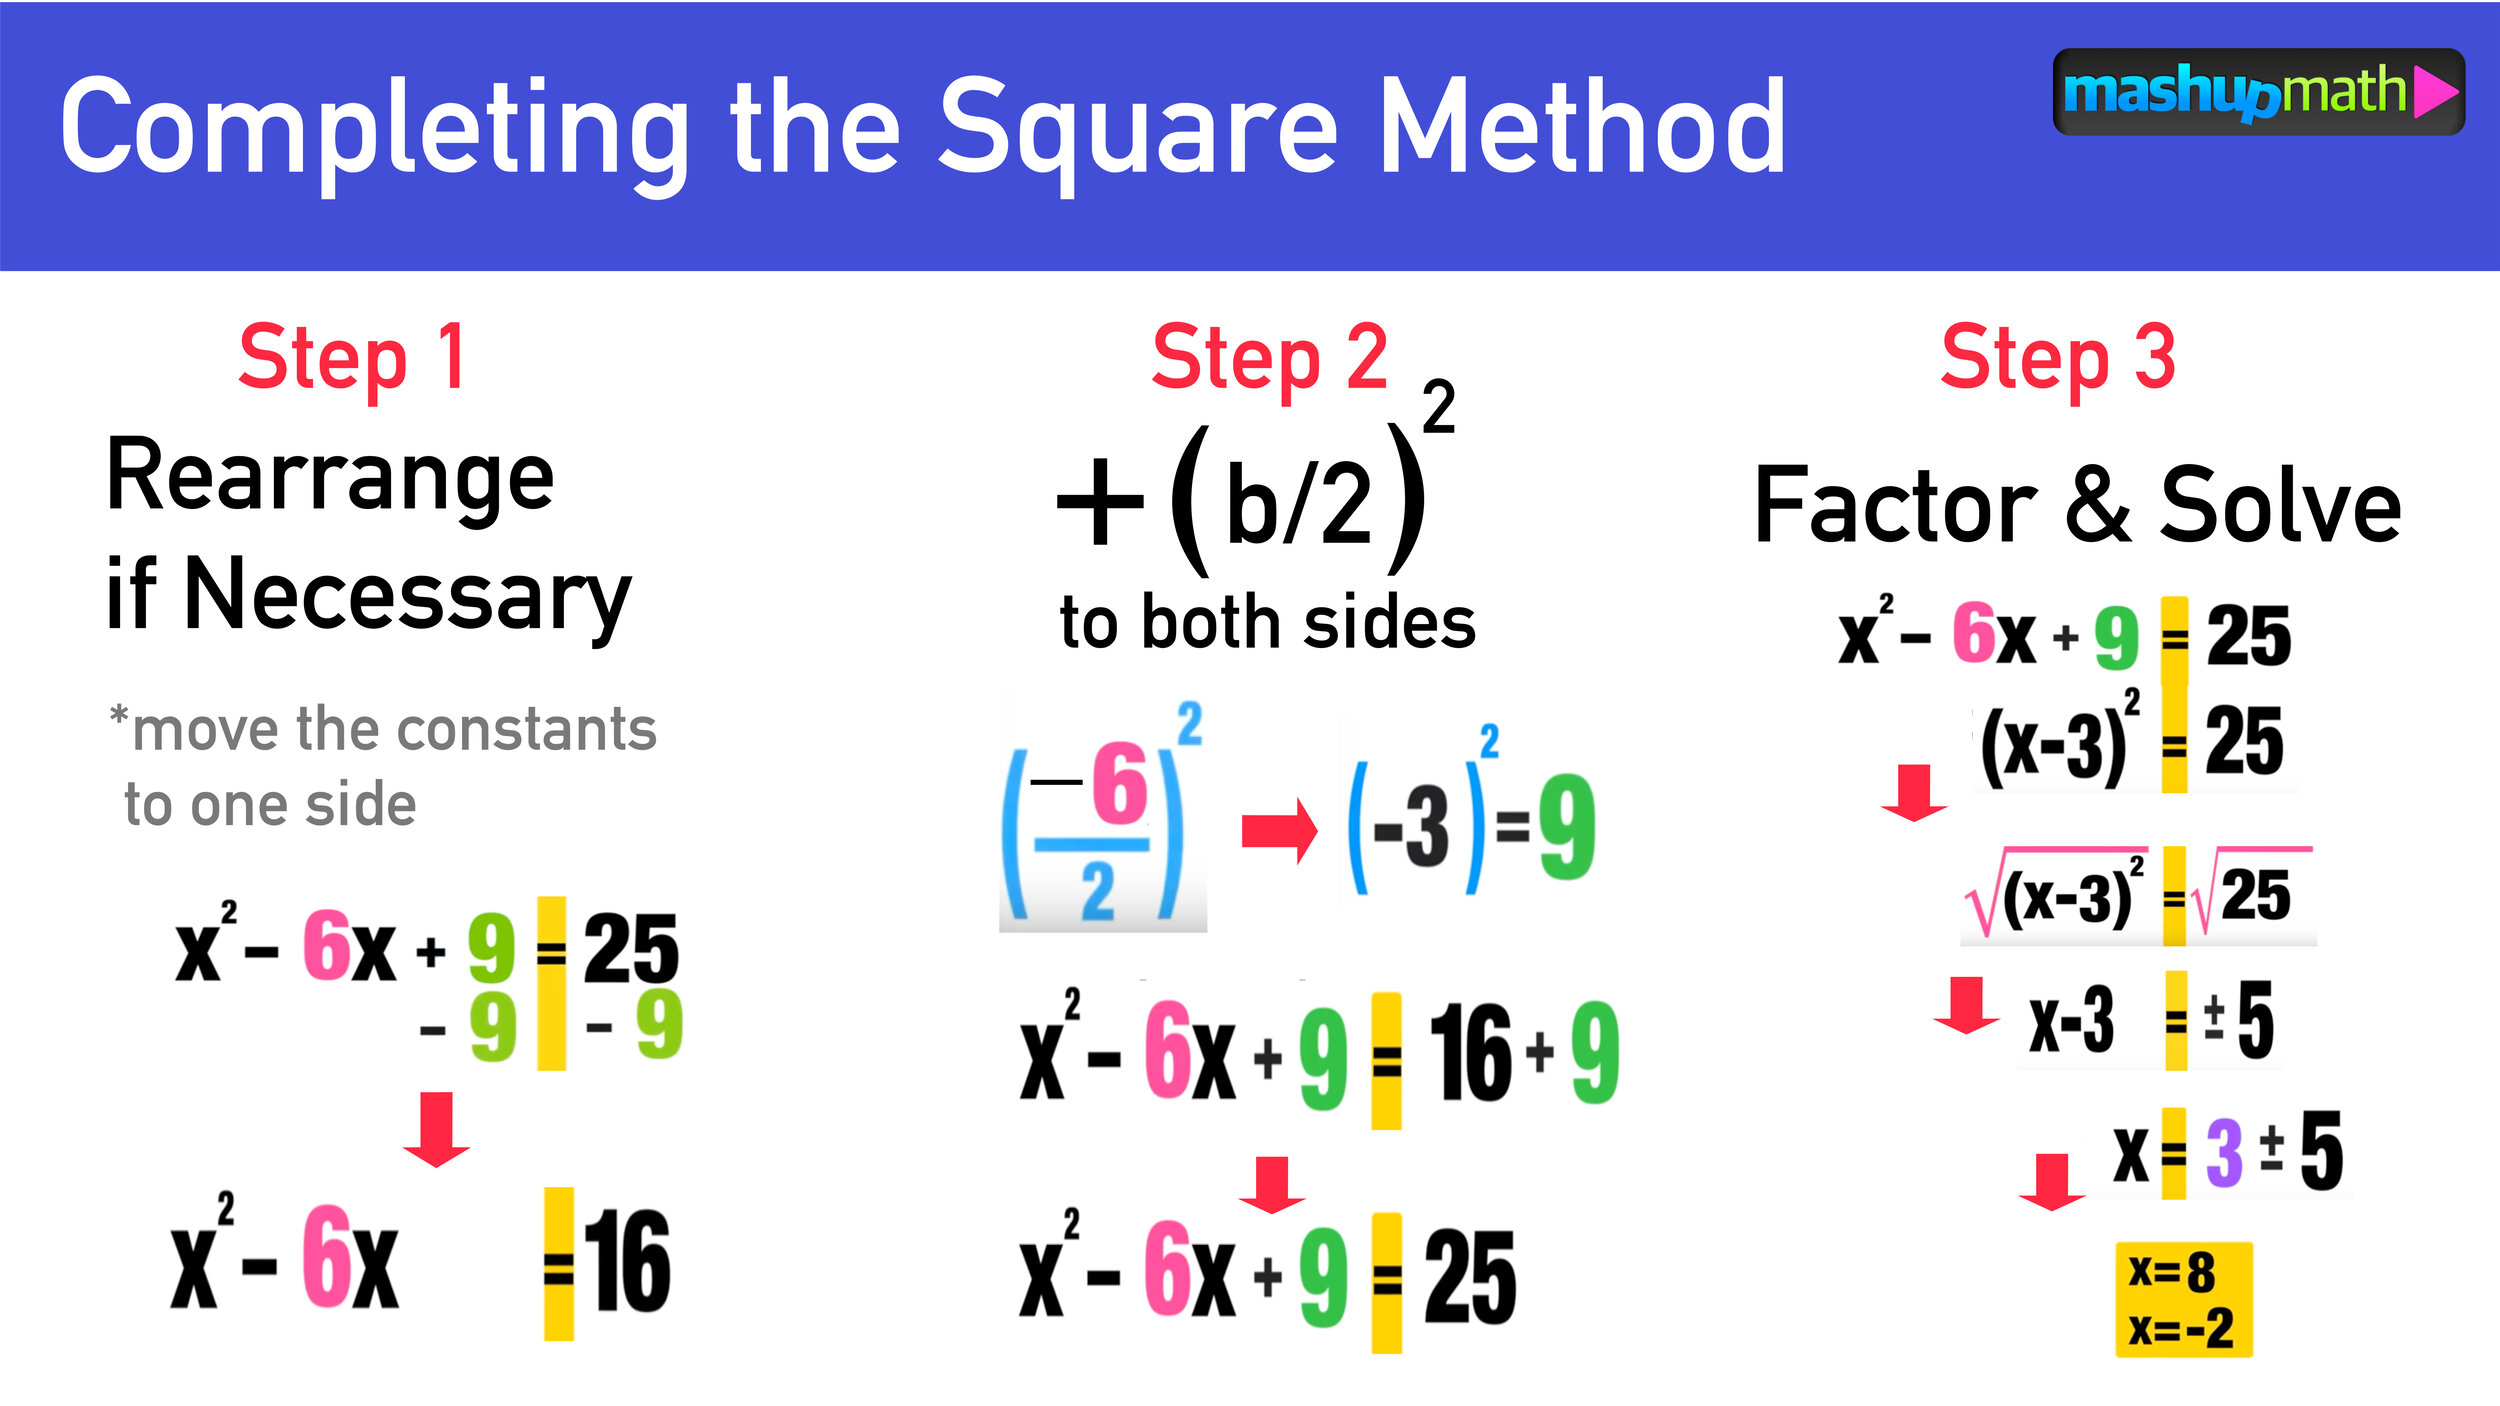
\includegraphics[scale=.65]{generalsquare.jpg}
	\caption{Credit: \url{https://www.mashupmath.com/blog/complete-the-square-formula}}
\end{figure}


\begin{figure}[ht]
	\centering
	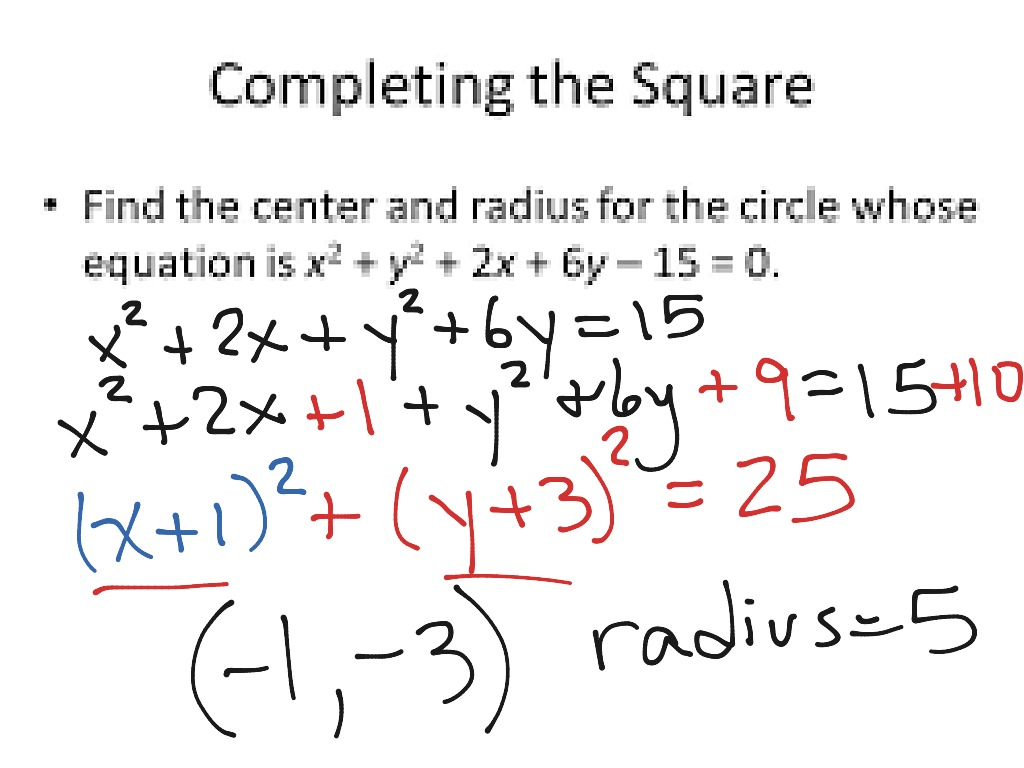
\includegraphics[scale=.25]{completecircle.jpg}
	\caption{Credit: \url{https://www.showme.com/sh/?h=nFTWVUG}}
\end{figure}

\section{Converting Between Radians and Degrees}

Here are the methods for converting between radians and degrees:

\[ \text{Radians} = \text{Degrees} \times \frac{\pi}{180} \]

\[ \text{Degrees} = \text{Radians} \times \frac{180}{\pi} \]

\section{Reference Angles}
We define reference angles as the smallest, positive, acute angle formed by the terminal side of an angle and the x-axis on a coordinate plane:\\

\begin{figure}[ht]
	\centering
	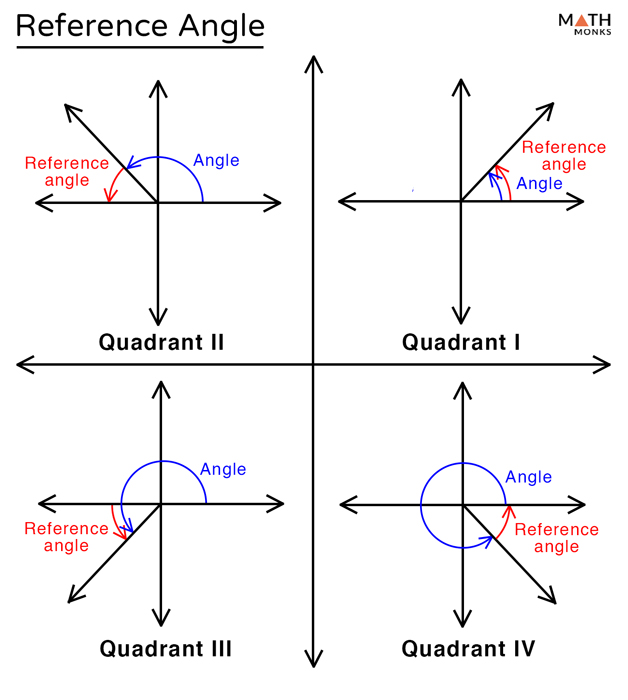
\includegraphics[scale=0.25]{Reference-Angle}
	\caption{Credit: \url{https://mathmonks.com/angle/reference-angle}}
\end{figure}

\section{Vertex of Quadratic}

Let \(f(x)=ax^2+bx+c\) where \(a\), \(b\), and \(c\) are constants. The vertex of \(f\) will always be\\

\[\left(\frac{-b}{2a}, f\left(\frac{-b}{2a}\right)\right)\]

\section{Factoring Higher-Degree Polynomials}

Let's suppose we have the equation \(8x^3+x+9\)=0. The left side isn't easily factorable and can't be plugged into the quadratic formula. Instead, we can find the possible rational zeros of the expression.\\

Let \(f(x)=a_nx^n+a_{n-1}x^{n-1}+...+a_2x^2+a_1x+a_0\) where  \(a\) are integers. Here,\\

\[\text{possible rational zeros}=\frac{\text{factors of }a_0\text{ (last term)}}{\text{factors of }a_n\text{(first term)}}\]

Hence, the possible rational zeroes of \(8x^3+x+9\) are \(\pm\frac{1,3,9}{1,2,4,8}=\pm\frac{1}{8},\pm\frac{1}{4}, \pm\frac{3}{8},\pm\frac{1}{2}, \pm\frac{3}{4},\pm1, \pm\frac{9}{8},\)

\(\pm\frac{3}{2}, \pm\frac{9}{4}, \pm\frac{9}{2},\pm3, \pm9\).\\


Personally, I like to start with integers. We can manually plug possible rational zeros in as \(x\). However, there's a trick to quickly evaluate polynomials at a certain value \(x\). This isn't easily explained in writing, so here's a helpful video from \href{https://www.youtube.com/watch?app=desktop&v=FxHWoUOq2iQ}{the Organic Chemistry tutor}. \\

Just remember that if \(f(a)=0\) than \((x-a)\) is a factor of \(f\).\\

\section{Intersection and Union}

The union is the combination of two sets, while the intersection is the overlap between two sets.\\

\begin{figure}[ht]
	\centering
	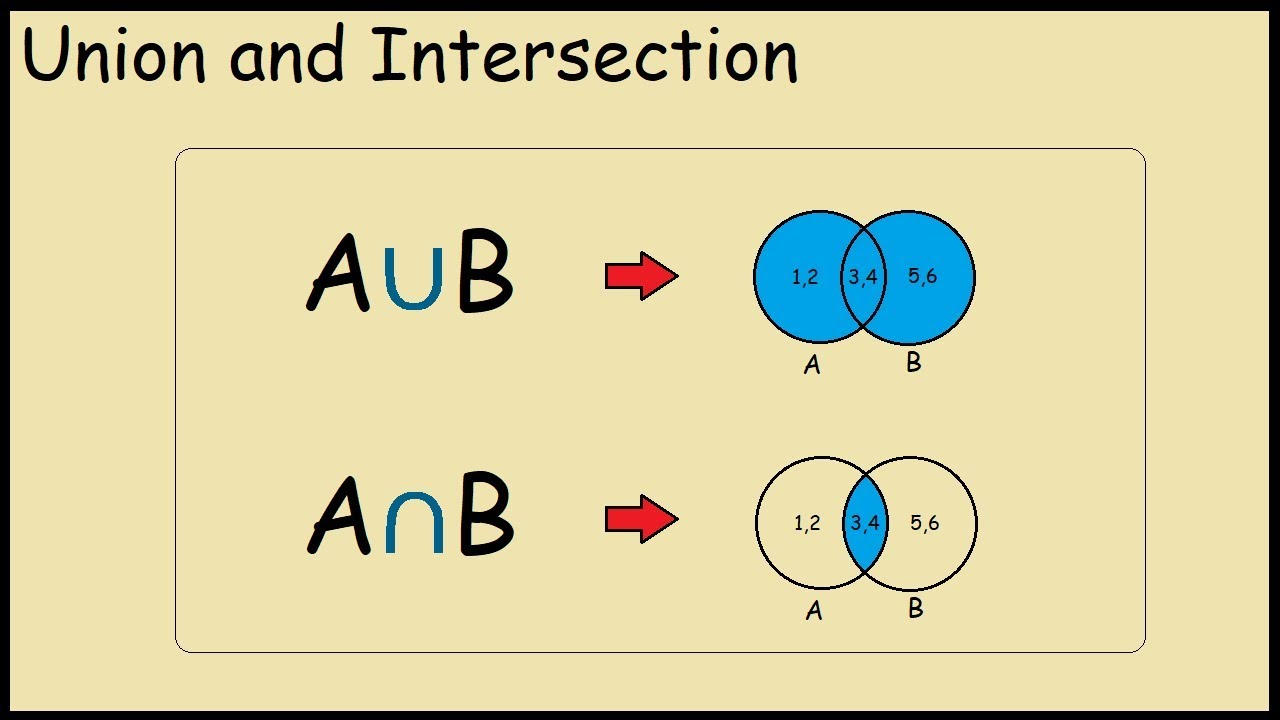
\includegraphics[scale=0.25]{intun}
	\caption{Credit: \url{https://www.youtube.com/watch?v=sdflTUW6gHo}}
\end{figure}


\end{document}
